\section{Introduction}

The MFA is a way of computer access control to secure data and applications,  in a way that a user must prove with two or more ways his identity. 
It can be with a password, a time-based one-time password\textbf{ (TOTP),} a digital certificate, or biometrics.

 Two-factor authentication \textbf{(2FA)} is a method that combines just two of the previously mentioned components.

\textbf{MFA} increases security because if just one of the credentials is compromised, the unauthorized user will not be able to know the MFA authentication requirement, and the access will be denied.


\subsection{How Multi-Factor Authentication Works?
}
As explained early in this document, MFA needs at least two credentials at login to verify the identity before granting access. Each additional layer of authentication to the login increases security.

MFA requires the combination of the following:


\begin{itemize}
\item \textbf{Something you Know}: Password, pin, or answer to security questions
\item \textbf{Something you Have}: Smart Card, Mobile token, hardware token.
\item \textbf{Something you Are}: Bio-metrics, voice recognition, fingerprint.
\end{itemize}

\newpage
\section{Requirements}
 
The IT requirements are the following:

\begin{itemize}
  \item Add and extra layer of security to the VPN connection.
  \item This can be an OTP or a "push" notification to an smartphone
  \item Compatibility with our systems
  \item Minor changes on our infrastructure for deployment
  \end{itemize}
  
  \newpage
  
  \section{Diagrams}
  
  \begin{figure}[!h]
      \centering
      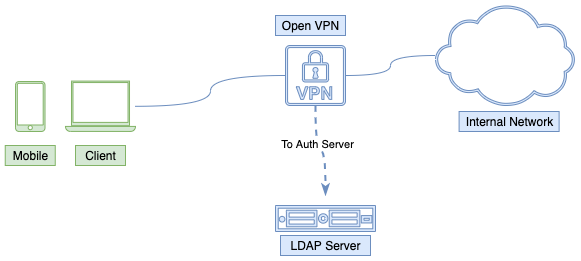
\includegraphics[width=160mm]{images/Pfsense - FreeIPA.drawio.png}
      \caption{OpenVPN + FreeIPA Authentication Server}
      \label{fig:label}
  \end{figure}
  
  
  
  \newpage
  \section{Alternatives}
  
  \subsection{FreeIPA + OTP}
  FreeIPA is a free and opensource Identity Managment System, aims to provide a centrally managed Identity, Policy and Audit (IPA)
  \subsection{DUO Authentication}
  \subsection{Comparison}
  
  \newpage
  \section{Final Toughs}



